\documentclass[11pt]{article}
% -----------------------------------------------------------------------------
% Response to the reviewers of MS CPENG-8674 (major revision, October 2026).
% Draft: answers are written only for the comments addressed so far.
% Code: MODULES/review29oct_fixed | Data: Data/06Nov_FINAL_SlabS10_7D_5sensors_5modes | Figures: ./figures_final
% Orange text = notes for the authors and placeholders (remove or fill before submission).
% -----------------------------------------------------------------------------
\usepackage[a4paper,margin=2.5cm]{geometry}
\usepackage{amsmath,amssymb,bm}
\usepackage{graphicx}
\usepackage{booktabs,multirow,array,longtable,tabularx}
\usepackage{xcolor}
\usepackage{caption,subcaption}
\usepackage{float}
\usepackage{enumitem}
\usepackage{titlesec}
\usepackage{tikz}
\usetikzlibrary{decorations.pathmorphing,arrows.meta,calc,positioning,patterns,decorations.pathreplacing}
\usepackage[colorlinks=true,linkcolor=blue!50!black,citecolor=blue!50!black,urlcolor=magenta]{hyperref}

\definecolor{resp}{RGB}{25,70,170}
\definecolor{note}{RGB}{205,95,0}
\linespread{1.15}
\setlength{\parindent}{0pt}
\setlength{\parskip}{4pt}
\captionsetup{font=small,labelfont=bf,labelsep=colon}
\renewcommand{\thetable}{R\arabic{table}}
\renewcommand{\thefigure}{R\arabic{figure}}
\renewcommand{\theequation}{R\arabic{equation}}
\titleformat{\section}{\normalfont\large\bfseries}{}{0pt}{}
\titleformat{\subsection}{\normalfont\bfseries}{}{0pt}{}
\setlist{itemsep=1pt,topsep=2pt}

% --- Comment / response / action blocks (as in our previous response letters) ---
\newenvironment{rcomment}[1]{\par\bigskip\noindent\textbf{Comment\ifx&#1&\else\ #1\fi:}\ \itshape}{\par}
\newenvironment{response}{\par\smallskip\noindent\color{resp}\textbf{Response:}\ }{\par}
\newenvironment{action}{\par\smallskip\noindent\color{resp}\textbf{Action:}\ }{\par}
\newcommand{\pending}{\par\smallskip\noindent\textcolor{gray}{\textbf{Response:} \textit{pending --- this comment
has not been addressed yet.}}\par}
\newcommand{\authornote}[1]{\textcolor{note}{\textsf{[Authors: #1]}}}
\newcommand{\tbd}[1]{\textcolor{note}{\textsf{[#1]}}}
\newcommand{\lines}[1]{\tbd{lines #1}}

\newcommand{\m}{\mathbf{m}}
\newcommand{\z}{\mathbf{z}}
\newcommand{\f}{\mathbf{f}}

\begin{document}

\begin{center}
{\Large\bfseries Response to reviewer comments}\\[8pt]
\textbf{MANUSCRIPT ID:} CPENG-8674\\
\textbf{Date:} \today\\
\textbf{Title:} Uncertainty-aware damage identification in short-span bridges via physics-informed variational
autoencoder\\
\textbf{Journal:} Journal of Computing in Civil Engineering
\end{center}

\noindent\fcolorbox{note}{note!6}{\parbox{\dimexpr\linewidth-2\fboxsep-2\fboxrule}{\small\color{note}\textsf{%
\textbf{Draft status (\today).} Answers are given only for the comments addressed so far; the other comments are
reproduced with the mark ``pending''. Orange text is for the authors: notes, and placeholders for the results of the
training on the final dataset and for the line numbers of the revised manuscript. All numbers in blue come from the
final dataset (\texttt{Data/06Nov\_FINAL\_SlabS10\_7D\_5sensors\_5modes}: bridge S10 of Moliner et al., 2017, as a beam on vertical elastic supports; five sensors, five modes) and the scripts in \texttt{MODULES/review29oct\_fixed} and
\texttt{MODULES/baseline\_GaussCopula\_GaussMarginals}.}}}

\bigskip
We would like to thank the three reviewers for the time and effort they devoted to conduct this insightful review.
In the following, we answer each comment point by point. Table~\ref{tab:summary} summarizes the responses and indicates where
the corresponding changes appear in the revised manuscript. Reviewer comments are reproduced in italics, and our responses and the resulting actions are written in blue.

% =============================================================================
\section{Summary of the responses}
% =============================================================================
{\small
\begin{longtable}{p{1.55cm}p{6.0cm}p{3.0cm}p{3.6cm}}
\caption{Point-by-point summary of the responses.}\label{tab:summary}\\
\toprule
Comment & Topic & Status & Revised manuscript \\
\midrule
\endfirsthead
\toprule
Comment & Topic & Status & Revised manuscript \\
\midrule
\endhead
R1.1 & Test data from a finer FE mesh & Addressed & \lines{xx--yy} \\
R1.2 & Model uncertainty and environmental variability & Addressed & \lines{xx--yy} \\
R1.3 & 95\% credible intervals and coverage & Addressed & \lines{xx--yy} \\
R1.4 & Comparison with Refs.\ 39 and 41 & Addressed & \lines{xx--yy} \\
R1.5 & Out-of-distribution test cases & Addressed & \lines{xx--yy} \\
R1.6 & Localized, mild and healthy cases; false positives & Addressed (results pending) & \lines{xx--yy} \\
R1.7 & Finer discretization and scalability & Addressed (results pending) & \lines{xx--yy} \\
R1.8 & Reference list & Addressed & \lines{xx--yy} \\
R2.1 & Utility for real bridges in the introduction & Addressed (draft) & \lines{xx--yy} \\
R2.2 & Realistic structure and elastic bearings & Addressed & \lines{xx--yy} \\
R2.3 & Damage parametrization, support conditions and detectable bearing damage & Addressed (VAE results pending) & \lines{xx--yy} \\
R2.4 & More realistic case study; laboratory beam & Partly addressed (no laboratory data) & \lines{xx--yy} \\
R3.1 & Robustness to modelling error (mass perturbation) & Addressed (results pending) & \lines{xx--yy} \\
R3.2 & Selection of $\gamma$ on the test set & Addressed (sensitivity study pending) & \lines{xx--yy} \\
R3.3 & Prior vs.\ sampling density of the training data & Addressed & \lines{xx--yy} \\
R3.4 & Number of modes and identifiability & Addressed (VAE results pending) & \lines{xx--yy} \\
R3.5 & Flowchart of the data generation and of the offline/online phases & Addressed & \lines{xx--yy} \\
R3.6 & Notation $\mathbf{K}_{\mathrm{G}}$ in Eq.~(11) & Pending & \\
R3.7 & Number of samples $H$ & Addressed & \lines{xx--yy} \\
R3.8 & Hardware and wall-clock time & Pending & \\
\bottomrule
\end{longtable}
}

% =============================================================================
\section{Reviewer \#1}
% =============================================================================
% The authors' notes on which these responses are based are kept in MODULES/_backup_09Nov_letter_user_notes/.

\begin{rcomment}{}
This paper presents a physics-informed Gaussian copula variational autoencoder for uncertainty-aware damage
identification using noisy natural frequencies and mode shapes. Replacing the learned decoder with a differentiable
eigensolver appears to be an interesting approach for end-to-end training, and the manuscript is clearly written. The work
builds on the authors' earlier Gaussian copula VAE (Reference 41) and extends it by embedding the eigensolver and
increasing the latent dimensionality from 2 to 5. The current validation is based on a single five-element synthetic
beam with measurement noise, and I believe that some additional evidence would further strengthen the conclusions
regarding uncertainty quantification, reliability, and scalability. Some clarifications are needed to better understand
the method and its applications.
\end{rcomment}

% -----------------------------------------------------------------------------
\begin{rcomment}{1}
The training and test data are generated using the same five-element model. Could the authors consider testing the trained model on observations generated from a finer mesh while retaining the same five damage zones and sensor locations as in the current paper? This would help assess robustness to model-form uncertainty, since field observations
may not necessarily be well represented by such a coarse discretization.
\end{rcomment}

\begin{response}
We have  built a new, more realistic case study, which also addresses the
concerns of Reviewer 2 (R2.2--R2.4). The bridge deck is discretized into 10 Euler--Bernoulli beam elements (two elements per damage zone) and rests on elastic bearings, represented by vertical springs at both ends (Fig.~\ref{fig:bridge}). 
We employ this 10-element model to generate the training and validation data.

The latent variables are one stiffness reduction factor per damage zone along the deck, as in the original submission, plus one stiffness factor per bearing (R2.2):
\begin{equation}
\hat{\mathbf{K}}_{\mathrm{G}}(\z)=\sum_{d=1}^{5} z_d\sum_{e\in\mathcal{Z}_d}\mathbf{K}_{e}
+z_{b,L}\,\mathbf{K}_{b,L}+z_{b,R}\,\mathbf{K}_{b,R},
\label{eq:Kz}
\end{equation}
where $\mathcal{Z}_d$ is the set of elements of zone $d$, and $\mathbf{K}_{b,L}$ and $\mathbf{K}_{b,R}$ contain the nominal stiffness of the left (L) and right (R) bearing springs.

For the testing phase, we generate the observations with a finer discretization of the same structure into 50 elements
of 0.2~m (ten per zone), with the same five damage zones, bearings and sensors (Fig.~\ref{fig:bridge}). The test damage
scenarios are also generated differently from the training ones (R1.5).
The performance metrics of the identification on the testing dataset are reported in Table~\ref{tab:metricsB} (R1.3).
\end{response}

% -----------------------------------------------------------------------------
\begin{rcomment}{2}
The introduction identifies model uncertainty, measurement error, and environmental variability as sources of
ill-posedness, whereas the numerical study focuses primarily on measurement noise. It would be useful to investigate how
the proposed framework handles the other sources of uncertainty or, alternatively, to discuss this point more explicitly
as a limitation of the present study.
\end{rcomment}

\begin{response}
We have extended the case study to account also for modeling error.
For that purpose, we have introduced a mass perturbation in the FE model used for training to account for discrepancies with respect to the nominal, reference properties of the system. 
The mass value of each structural element is independently perturbed as: 
\begin{equation}
	m_e^{\text{true}} = m_e^{\text{nom}} \left(1 + \epsilon \xi_e\right), \quad e = 1, \dots, n_{\text{e}},
	\label{eq:modeling_error}
\end{equation}
where $m_e^{\text{nom}}$ denotes the nominal mass value at the $e$-th element, with $n_{e}$ total elements; $\xi_e$ is an independent sample from a standard Gaussian random variable; and $\epsilon$ is the model-error level. 
In this work, we assing a $\epsilon = 0.05$ to represent a $5\%$ error. 
Besides, we account for the FE discretization error by employing a finer mesh to generate the test dataset (50-element model as indicated in R1.1). 

A realistic description of environmental and opeational effects requires long-term monitoring data, which cannot be reproduced reliably in the current synthetic dataset. 
We now include in the introduction the sources of uncertainty handled in the present work. 
Besides, in the conclusions, we describe in more detail the limitations and acknowledge the lack of environmental variability. 
We propose in the conclusions (future work**) an experimental validation strategy to incorporate this source of uncertainty as future work.


%
%We agree that measurement noise is not the only source of uncertainty in practice. The revised study accounts for the
%following sources:
%\begin{enumerate}[leftmargin=*,label=(\alph*)]
%\item \emph{Measurement error.} As in the original submission, the natural frequencies and mode shapes are corrupted
%with Gaussian noise (2.5\% of the frequencies and 5\% of the peak amplitude of the mode shapes).
%\item \emph{Modelling error.} The data are generated with a model that differs from the one used by the SciML method. The
%mass of each 1~m segment of every simulated structure is perturbed as
%\begin{equation}
%\mathbf{M}_e^{\mathrm{data}}=(1+\mu_{s(e)})\,\mathbf{M}_e,\qquad \mu_{s}\sim\mathcal{N}(0,0.05^2),
%\label{eq:asbuilt}
%\end{equation}
%where $s(e)$ is the segment of element $e$, whereas the decoder keeps the nominal mass matrix. Uncertain permanent loads are
%also considered in dynamic studies of short-span bridges (e.g., $\pm30\%$ of the ballast thickness in Moliner et al.,
%2017). In addition, the test data are generated with a finer discretization (50 elements, R1.1) to explore the robustness
%against model-form error.
%\item \emph{Limited information.} We also explore the effect of a scarce measurement data by reducing the number of identified modes (three instead of five), as also requested by Reviewer 3 (R3.4).
%\item \emph{Environmental and operational variability.} A realistic description of these effects requires long-term
%monitoring data, which cannot be reproduced reliably in a synthetic dataset. We acknowledge this as a limitation of the
%present validation and propose an experimental validation that incorporates this source of uncertainty as future work.
%\end{enumerate}

%The statistics of the measurement and modelling errors are estimated by simulation and included in the likelihood (R1.3).
%Note that the objective of the present work is not to disentangle these sources of uncertainty (i.e., to quantify the  contribution of each one), which could be addressed in future work, but to include them to offer a realistic case study
%and a reliable validation.
\end{response}

%\begin{action}
%New paragraph on the sources of uncertainty \lines{xx--yy}, with Eq.~\tbd{x} (Eq.~\eqref{eq:asbuilt}); environmental
%and operational variability discussed as a limitation in the conclusions \lines{xx--yy}.
%\end{action}

% -----------------------------------------------------------------------------
\begin{rcomment}{3}
The abstract reports 77.2\% coverage (line 32), whereas line 352 reports a value of 0.789 for nominal 95\% intervals.
Could the authors clarify how these two values are related? A value below 80\% for nominal 95\% intervals may indicate
some undercoverage. A brief discussion of how the uncertainty intervals are calibrated would therefore be helpful.
\end{rcomment}
\begin{response}
	We have entirely updated the results section according to the new case study and generated datasets.
	In addition, we found an error in the 95\% coverage calculation of the submitted version, which produced the undercoverage results.
	We have fixed this error and now include the detailed formulation of the metrics used to evaluate the performance, and a table (Table ** in the revised manuscript) that summarizes the results. 
	
	For each test observation $\m_t$ ($t=1,\dots,N$) and stiffness factor $z_d$ ($d=1,\dots,D$), with true value
	$z^*_{t,d}$, the VAE provides a marginal posterior: a Gaussian distribution with location $\mu_{t,d}$ and scale
	$\sigma_{t,d}$, truncated to the interval of interest $[z_{\text{lb}},z_{\text{ub}}]$, with density and cumulative distribution function (CDF)
	\begin{equation}
		q_{t,d}(z)=\frac{\varphi\big((z-\mu_{t,d})/\sigma_{t,d}\big)}{\sigma_{t,d}\,Z_{t,d}},\qquad
		F_{t,d}(z)=\frac{\Phi\big((z-\mu_{t,d})/\sigma_{t,d}\big)-\Phi\big((z_{\text{lb}}-\mu_{t,d})/\sigma_{t,d}\big)}{Z_{t,d}},
		\label{eq:marginal_tn}
	\end{equation}
	where $Z_{t,d}=\Phi\big((z_{\text{ub}}-\mu_{t,d})/\sigma_{t,d}\big)-\Phi\big((z_{\text{lb}}-\mu_{t,d})/\sigma_{t,d}\big)$, and $\varphi$ and
	$\Phi$ are the standard normal density and CDF. Every metric is averaged over the $N\times D$ stiffness factors of the
	test set:
	\begin{itemize}[leftmargin=*]
		\item \emph{Mean squared error (MSE) and mean absolute error (MAE)} of the point estimate $\hat z_{t,d}$, which is the
		mean of the marginal posterior of Eq.~\eqref{eq:marginal_tn}:
		\begin{equation*}
			\hat z_{t,d}=\int_{z_{\text{lb}}}^{z_{\text{ub}}} z\,q_{t,d}(z)\,\mathrm{d}z
			=\mu_{t,d}+\sigma_{t,d}\,\frac{\varphi\big((z_{\text{lb}}-\mu_{t,d})/\sigma_{t,d}\big)-\varphi\big((z_{\text{ub}}-\mu_{t,d})/\sigma_{t,d}\big)}{Z_{t,d}},
		\end{equation*}
		\begin{equation}
			\mathrm{MSE}=\frac{1}{ND}\sum_{t=1}^{N}\sum_{d=1}^{D}\big(\hat z_{t,d}-z^*_{t,d}\big)^2,\qquad
			\mathrm{MAE}=\frac{1}{ND}\sum_{t=1}^{N}\sum_{d=1}^{D}\big|\hat z_{t,d}-z^*_{t,d}\big|.
			\label{eq:mse_mae}
		\end{equation}
		\item \emph{Average log-likelihood} of the true values under the marginal posteriors:
		\begin{equation}
			\mathrm{ALL}=\frac{1}{ND}\sum_{t=1}^{N}\sum_{d=1}^{D}\log q_{t,d}\big(z^*_{t,d}\big).
			\label{eq:all}
		\end{equation}
		\item \emph{Coverage}: fraction of the true values that lie inside the central credible interval of level $p$, i.e.,
		between the $(1-p)/2$ and $(1+p)/2$ quantiles of the marginal posterior:
		\begin{equation}
			C(p)=\frac{1}{ND}\sum_{t=1}^{N}\sum_{d=1}^{D}\mathbb{I}\Big[\frac{1-p}{2}\le F_{t,d}\big(z^*_{t,d}\big)\le\frac{1+p}{2}\Big],
			\label{eq:coverage}
		\end{equation}
		where $\mathbb{I}[\cdot]$ equals 1 if the condition holds and 0 otherwise. The 95\% coverage is $C(0.95)$. If the
		posterior is calibrated, $C(p)\approx p$; a lower value (undercoverage) means that the true values fall outside the
		intervals more often than their level indicates.
		\item \emph{Mean absolute calibration error} over 19 levels, $p_l=0.05,0.10,\dots,0.95$:
		\begin{equation}
			\mathrm{MACE}=\frac{1}{19}\sum_{l=1}^{19}\big|C(p_l)-p_l\big|.
			\label{eq:mace}
		\end{equation}
	\end{itemize}
	The credible intervals are not recalibrated after training: they are the central quantiles of the marginal posteriors
	predicted by the VAE, and Eqs.~\eqref{eq:coverage} and \eqref{eq:mace} evaluate their calibration.

%	In the submitted version, due to a programming error, the 95\% coverage was computed as
%	\begin{equation*}
%		C_{\text{submitted}}=\frac{1}{N^2D}\sum_{t=1}^{N}\sum_{t'=1}^{N}\sum_{d=1}^{D}
%		\mathbb{I}\big[\mu_{t,d}-1.96\,\sigma_{t,d}\le z^*_{t',d}\le\mu_{t,d}+1.96\,\sigma_{t,d}\big],
%	\end{equation*}
%	i.e., the interval of each test observation $t$ was evaluated at the true values $z^*_{t',d}$ of all the $N$ test
%	observations, instead of only at its own true values ($t'=t$) as in Eq.~\eqref{eq:coverage}. Besides,
%	$\mu_{t,d}\pm1.96\,\sigma_{t,d}$ are the bounds of the 95\% interval of the Gaussian distribution before its
%	truncation to $[z_{\text{lb}},z_{\text{ub}}]$, whereas Eq.~\eqref{eq:coverage} uses the quantiles of the truncated
%	distribution.

	Table~\ref{tab:metricsB} reports the metrics on the test dataset: 87.2\% of the true stiffness factors lie inside their 95\%
	credible intervals (87.9\% of the damaged ones and 86.8\% of the undamaged ones), and the MACE is 0.124.
	
	\begin{table}[H]
		\centering\small
		\caption{Performance metrics, Eqs.~\eqref{eq:mse_mae}--\eqref{eq:mace}, on the test dataset (1\,200 observations with seven
			stiffness factors each).}
		\label{tab:metricsB}
		\begin{tabular}{lccc}
			\toprule
			Metric & All stiffness factors & Damaged ($z^*<0.95$) & Undamaged ($z^*\ge0.95$) \\
			\midrule
			MSE & 0.00715 & 0.00834 & 0.00656 \\
			MAE & 0.0648 & 0.0668 & 0.0638 \\
			ALL & 1.515 & 1.050 & 1.744 \\
			MACE & 0.124 & 0.070 & 0.151 \\
			95\% coverage, $C(0.95)$ & 0.872 & 0.879 & 0.868 \\
			\bottomrule
		\end{tabular}
	\end{table}
\end{response}


%

% -----------------------------------------------------------------------------
\begin{rcomment}{4}
References 39 (Gaussian mixture autoencoder) and 41 (Gaussian copula VAE) introduce closely related methods that could
potentially serve as useful baselines. A comparison with these approaches would help assess the benefits of the proposed
strategy more effectively.
\end{rcomment}

\begin{response}
	The proposed method builds on two previous works of the authors, Ref.~39 (Gaussian mixture autoencoder) and Ref.~41 (Gaussian copula VAE).
	In both works, the forward operator is approximated with a neural network (surrogate model) that is pre-trained and subsequently frozen while the encoder is trained.
	This approach provided good results in our previous works.
	However, it adds an extra source of uncertainty by approximating the forward operator, compared to embedding the governing law, which endows interpretability to the data-driven model. 
	Besides, the adequate performance of the surrogate decoder depends on the design of experiments conducted to generate the training data.
	Finally, this strategy demands a two-step training strategy, where the surrogate decoder is first approximated. 
	
	To quantify these differences, we have implemented the approach of Ref.~41 for the present problem: the eigenvalue solver is replaced by a surrogate NN. The rest of the architecture is unchanged.
	Table~\ref{tab:surrogate} compares the key properties and results for the surrogate approach against the proposed method.
	Both approaches reach practically the same values of all the performance metrics, i.e., they identify the damage and quantify its uncertainty with the same accuracy. This is because, trained with the 14,000 simulations of the training dataset, the surrogate is accurate in the whole domain of these data: at the damage states of the test dataset, its frequencies differ from those of the eigenvalue solver by at most 1.3\%, less than the measurement noise (2.5\%).
	However, with the eigenvalue solver, the approximate posterior is closer to the exact Bayesian posterior for 67\% of the test observations, and the lower bound of the Kullback--Leibler divergence from the exact posterior is 5\% smaller (0.114 against 0.120).
	This difference is small but statistically significant: per test observation, the Kullback--Leibler divergence from the exact posterior is larger with the surrogate by $0.008\pm0.002$ (mean $\pm$ standard error over the 1,200 observations, paired comparison with the exact model). The posterior of the proposed method is also closer to the exact posterior in 10 of the 11 benchmark scenarios of the manuscript, whose posteriors are plotted.

	\begin{table}[H]
		\centering\small
		\caption{Comparison of the proposed method (eigenvalue solver) with the approach of Ref.~41 (surrogate decoder), with
			the same training data, encoder, posterior model, likelihood and training protocol. Performance metrics as defined
			in R1.3.}
		\label{tab:surrogate}
		\begin{tabular}{lcc}
			\toprule
			& Proposed (eigenvalue solver) & Ref.~41 (surrogate decoder) \\
			\midrule
			\multicolumn{3}{l}{\emph{Learnable parameters}} \\
			\quad Encoder & 75,306 & 75,306 \\
			\quad Decoder & -- & 13,640 \\
			\quad Total & 75,306 & 88,946 \\
			\midrule
			\multicolumn{3}{l}{\emph{Performance metrics}} \\
			\quad MSE & 0.00715 & 0.00715 \\
			\quad MAE & 0.0648 & 0.0647 \\
			\quad ALL & 1.515 & 1.517 \\
			\quad MACE & 0.124 & 0.124 \\
			\quad 95\% coverage, $C(0.95)$ & 0.872 & 0.872 \\
			\bottomrule
		\end{tabular}
	\end{table}

	Therefore, the advantage of embedding the physics is not a higher accuracy, but that this accuracy is reached without approximating the forward operator:
	\begin{itemize}[leftmargin=*]
		\item \emph{Physical meaning of the latent variables.} The decoder is the FE model itself: the latent variables scale the stiffness matrices of the damage zones and bearings (Eq.~\eqref{eq:Kz}), and the decoder solves the eigenvalue problem of the resulting model for any damage state. Hence, the identified variables are exactly the stiffness factors that explain the measurements, whereas with a surrogate they are the inputs of a black-box approximation, whose accuracy depends on its training data. Moreover, inside its training domain the surrogate reproduces the frequencies of the eigenvalue solver within 0.2\% on average, but their sensitivities to the stiffness factors, $\partial f/\partial z_d$, which drive the training of the encoder, only within 15\% (median relative error at 2,000 damage states); the eigenvalue solver provides them exactly.
		\item \emph{Physically consistent predictions.} The eigenvalue solver satisfies the physical laws of the FE model by construction, whereas the surrogate only approximates them (Fig.~\ref{fig:physics}). First, increasing the stiffness of a zone or bearing can never lower a natural frequency (Rayleigh's principle), but the surrogate predicts a lower frequency for a 5\% stiffer zone or bearing in 1.4\% of the combinations of damage state, parameter and mode (8.2\% and 14.3\% when it is trained with 2,000 and 500 simulations). Second, the bridge is symmetric, so two mirror-image damage scenarios have identical frequencies, but the surrogate assigns them frequencies that differ by 0.21\% on average and by up to 3.1\%, i.e., more than the measurement noise.
		\item \emph{Validity for any damage state.} The eigenvalue solver is exact outside the training domain, whereas the surrogate is not (Table~\ref{tab:forward}): when one deck zone is damaged beyond the lower bound of the training data ($z_d\in[0.20,0.45)$) or the bearings are stiffer than nominal ($z_{b}\in(1,3]$), the frequencies of the surrogate differ from those of the eigenvalue solver by more than the measurement noise (2.5\%) in 50\% and 93\% of the damage states, respectively, and by up to 18\% and 31\%. Therefore, the surrogate cannot be used beyond its training domain without generating new data and training it again.
		\item \emph{Single training step.} The proposed method does not require generating training data for a surrogate, selecting its architecture and training it, or retraining it when the FE model, the sensor layout or the selected modes change. It also has 15\% fewer learnable parameters (75,306 against 88,946).
		\item \emph{No data needed for the forward operator.} The accuracy of the surrogate depends on the number of simulations used to train it: with 2,000 or 500 simulations instead of the 14,000 of the training dataset, its mean error grows from 0.19\% to 0.57\% and 0.99\%, and the share of damage states in which it exceeds the measurement noise grows from 0.1\% to 3.5\% and 18\% (Table~\ref{tab:forward}). The eigenvalue solver needs no data to be exact.
	\end{itemize}
	\begin{table}[H]
		\centering\small
		\caption{Difference between the natural frequencies computed by the surrogate decoder (architecture of Ref.~41) and
			by the eigenvalue solver of the proposed method, which is exact for the FE model: mean, 95th percentile and maximum
			over all modes and damage states, and share of damage states in which the difference of at least one frequency
			exceeds the measurement noise (2.5\%). The training domain is $[0.45,1]^7$.}
		\label{tab:forward}
		\footnotesize
		\begin{tabular}{llcccc}
			\toprule
			Damage states & Simulations & Mean & 95th perc. & Max. & Above noise \\
			\midrule
			Inside the training domain & 14,000 & 0.19\% & 0.50\% & 4.3\% & 0.1\% \\
			 & 5,000 & 0.28\% & 0.75\% & 5.2\% & 0.4\% \\
			 & 2,000 & 0.57\% & 1.60\% & 6.9\% & 3.5\% \\
			 & 1,000 & 0.76\% & 2.21\% & 7.8\% & 9.1\% \\
			 & 500 & 0.99\% & 2.94\% & 15.1\% & 17.7\% \\
			\midrule
			One deck zone with $z_d\in[0.20,0.45)$ & 14,000 & 1.45\% & 5.45\% & 18.3\% & 49.9\% \\
			Bearings with $z_b\in(1,3]$ & 14,000 & 4.63\% & 12.47\% & 31.2\% & 93.4\% \\
			\bottomrule
		\end{tabular}
	\end{table}
	\begin{figure}[H]
		\centering
		\includegraphics[width=\textwidth]{figures_final/Fig_surrogate_physics.pdf}
		\caption{Physical laws that the eigenvalue solver satisfies by construction and the surrogate decoder does not (20,000 damage states drawn uniformly over the training domain). (a) Frequency of mode 2 vs the stiffness factor of zone 1, with the other factors fixed at $(z_2,\dots,z_5,z_{b,L},z_{b,R})=(0.45,0.65,0.48,0.80,0.48,0.49)$: the case with the most decreasing steps of the surrogate among 2,100 random sweeps. (b) Share of cases in which a 5\% stiffer zone or bearing gets a lower natural frequency, which is impossible (Rayleigh's principle). (c) Mean difference between the frequencies of mirror-image damage scenarios, which are identical in the symmetric bridge.}
		\label{fig:physics}
	\end{figure}
	\authornote{Running on goliat (data-budget runs): both approaches trained with 500 and 1,000 simulations. Add their performance metrics here.}
	Once trained, both approaches identify the damage with the encoder only, at the same cost.

	The revised manuscript (Section Results and discussion) includes a new table that compares both approaches with the performance metrics of R1.3 (MSE, MAE, ALL, MACE and 95\% coverage) and with their learnable parameters, as in Table~\ref{tab:surrogate}.

	%In Ref.~39, the true posterior is approximated with a Gaussian mixture. This approach has been extensively compared to Gaussian copulas in the recent Ref.~41, where the results revealed the copula able to reach an accuracy comparable to that of Gaussian mixtures with full covariance matrix at a lower computational cost. 
	%This advantange augments as the dimensionality (D) of the latent space increases.
	%For the present case study with seven latent variables, a mixture of $K=5$ Gaussians with full covariance matrices requires $K\,(1+D+D(D+1)/2)-1=179$ parameters to describe the posterior, against $2D+D(D-1)/2=35$ for the Gaussian copula, and its truncation to the support of the prior involves the joint seven-dimensional distribution instead of seven one-dimensional marginals. 
	%For these reasons, the authors consider the comparison against Gaussian mixtures sufficiently analyzed to support the decision of using copulas, and will not include it here.
	
	
	%	
	%The proposed method builds on two previous works of the authors, Ref.~39 (Gaussian mixture autoencoder) and Ref.~41
	%(Gaussian copula VAE), and differs from them in two components (Table~\ref{tab:refs}):
	%\begin{enumerate}[leftmargin=*,label=(\roman*)]
	%\item \emph{Decoder.} Refs.~39 and 41 approximate the forward operator with a neural network (surrogate model) that is
	%pre-trained on simulated data and then frozen while the encoder is trained. The proposed method embeds a differentiable
	%eigenvalue solver that computes the forward problem exactly, without trainable parameters and without a pre-training
	%step.
	%\item \emph{Posterior model.} Ref.~39 describes the posterior with a Gaussian mixture, whereas Ref.~41 and the proposed
	%method use a Gaussian copula.
	%\end{enumerate}
	%
	%\textit{Comparison with Ref.~41 (decoder).} Since Ref.~41 and the proposed method share the posterior model, a comparison
	%with Ref.~41 isolates the effect of the decoder. We implemented the approach of Ref.~41 for the present problem: the
	%eigenvalue solver is replaced by a fully connected surrogate with the architecture of Ref.~41, which is first trained, at
	%the damage states of the same training dataset, to reproduce the natural frequencies and mode shapes computed with the FE
	%model. Its weights are then frozen,
	%and the encoder is trained exactly as in the proposed method (same dataset, encoder, posterior model, likelihood and
	%training protocol). The surrogate introduces an additional approximation error in the forward model, which the likelihood
	%does not account for, and requires a second training step and additional parameters. We compare both approaches in terms of
	%the accuracy of the decoder, the agreement of the approximate posterior with the exact posterior, the metrics of the
	%manuscript on both test sets, and the computational cost (Table~\ref{tab:surrogate}).
	%
	%
	%\textit{Comparison with Ref.~39 (posterior model).} Gaussian mixtures and the Gaussian copula were already compared in
	%Ref.~41: the copula reached an accuracy comparable to that of Gaussian mixtures with full covariance matrices at a lower
	%computational cost, mixtures with diagonal covariance matrices were less accurate because they cannot capture the
	%correlations between the latent variables, and increasing the number of mixture components did not improve the results.
	%The differences grow with the dimension $D$ of the latent space. For the seven latent variables of the revised case study, a
	%mixture of $K=5$ Gaussians with full covariance matrices requires $K\,(1+D+D(D+1)/2)-1=179$ parameters per observation,
	%against $2D+D(D-1)/2=35$ for the Gaussian copula, and its truncation to the support of the prior involves the joint
	%seven-dimensional distribution instead of seven one-dimensional marginals. For these reasons, we do not repeat this
	%comparison here, and the revised manuscript summarizes the findings of Ref.~41.
	
	
\end{response}


% -----------------------------------------------------------------------------
\begin{rcomment}{5}
All test cases appear to be sampled from the same distribution as the training data. It would be helpful to include several additional cases where the test data fall outside the training distribution to illustrate how the proposed method behaves under distribution shift.
\end{rcomment}

\begin{response}
In the revised study, all the test scenarios fall outside the training distribution, since they are generated
differently from the training and validation scenarios. Besides the finer discretization of the test data (50 elements
instead of 10, R1.1), we create the damage scenarios differently with an equivalent stiffness reduction:
\begin{itemize}[leftmargin=*]
\item \emph{Train/validation data (10-element model).} The stiffness reduction factor $z_d$ multiplies the bending stiffness of the elements in zone $d$ (Eq.~\eqref{eq:Kz}), so the damage is spread uniformly over the entire zone. 

\item \emph{Test dataset (finely discretized FE model with 50 elements).} Each test scenario is defined by stiffness factors $z_d$ drawn from the same design of experiments as the training data (R1.6), but in every damaged zone ($z_d<0.95$) the loss of stiffness is concentrated in a damaged region of length $\ell_d$, at a random position within the zone, while the rest of the zone keeps its nominal stiffness.
The stiffness factor $s$ of the damaged region is set so that the zone keeps the same stiffness of a zone uniformly damaged with factor $z_d$.
For a zone of length $L_z$ and nominal bending stiffness $EI$ subjected to a constant bending moment $M$, the relative rotation between its ends is $\theta=M\int_{L_z}\mathrm{d}x/EI(x)$, so both zones have the same flexibility if
\begin{equation}
\frac{L_z}{z_d\,EI}=\frac{\ell_d}{s\,EI}+\frac{L_z-\ell_d}{EI}
\qquad\Longrightarrow\qquad
s=\frac{\alpha\,z_d}{1-(1-\alpha)\,z_d},\qquad\text{with}\quad\alpha=\frac{\ell_d}{L_z}.
\label{eq:localized}
\end{equation}
Namely, $z_d$ is the equivalent stiffness factor of the zone, regardless the distribution of damage within the zone.
A uniformly damaged zone ($\alpha=1$, as considered to create the training data) gives $s=z_d$, whereas a shorter damaged region requires a larger local loss of stiffness.
For instance, a zone with $z_d=0.6$ may be damaged over 0.4~m ($\alpha=0.2$, $s=0.23$), over 1.0~m ($\alpha=0.5$, $s=0.43$) or over the whole zone ($\alpha=1$, $s=0.60$).
In the 50-element model, the damaged region consists of $n$ contiguous elements of 0.2~m, so $\alpha=n/10$ ($L_z=2$~m).
The number of damaged elements $n$ is drawn uniformly among the values that keep $s\ge0.15$ (max. 85\% of local stiffness loss), so severe damage cannot be concentrated in a very short region (e.g., at least three elements, i.e., 0.6~m, for $z_d=0.45$), and the position of the damaged region within the zone is also drawn uniformly.
Undamaged deck zones and bearings are imposed as in the training data.
\end{itemize}
This approach allows us to describe more realistic scenarios in the testing dataset, such as the effect of cracking
(localized loss of stiffness), while preserving a controlled design of experiments for training. All the test results
of the revised manuscript (e.g., Tables~\ref{tab:metricsB} and~\ref{tab:surrogate}), including the benchmark scenarios
whose posteriors are plotted, are obtained with these out-of-distribution test scenarios.
\end{response}

\begin{action}
Generation of the test scenarios with localized damage (Eq.~\eqref{eq:localized}) \lines{xx--yy}.
\end{action}

% -----------------------------------------------------------------------------
\begin{rcomment}{6}
The paper introduces damage by sampling from a uniform distribution (line 323), which appears to result in substantial
stiffness reduction in most or all five elements simultaneously. Since structural damage is often localized, it would be
valuable to also evaluate healthy cases and cases with mild damage affecting only one or two elements. Reporting the
corresponding false-positive behavior would further support the manuscript's emphasis on early damage identification.
\end{rcomment}

\begin{response}
Following this comment, we generated a new dataset whose design of experiments (DoE) focuses on localized damage, while
still including the uniform sampling of the original submission. The DoE is a stratified mixture of scenario categories
(Table~\ref{tab:doe}): healthy structures, damage at one, two, three, or four to five locations, and a category drawn
uniformly over the whole parameter space. Within each category, every damage location (five zones and two bearings) and
every combination of locations appears the same number of times. The stiffness factors of the damaged parameters are
stratified (Latin hypercube sampling) over $[0.45,0.95)$, which covers mild to severe damage, and the undamaged
parameters lie in $[0.95,1]$. The validation and test sets follow the same proportions.

The first eleven test samples are benchmark scenarios: a healthy bridge (P0), damage in a single zone with severe,
moderate, mild and very mild severity (P1, P2, P3 and P10, the latter with $z_4=0.90$), degradation of one bearing (P4),
and combined scenarios (P5 to P9).

To quantify false positives, a parameter is declared damaged when the upper limit of its 95\% credible interval falls
below the damage threshold 0.95. We report the false-alarm rate (fraction of undamaged parameters declared damaged) and the
detection rate (fraction of parameters with $z^*<0.90$ declared damaged) on test set B. The false-alarm rate is 3.2\%
(2.0\% for the deck zones and 6.3\% for the bearings). In the healthy scenarios, it is 1.9\%, and 15 of the 120 healthy
structures (12.5\%) show at least one false alarm. The detection rate is 66.6\%, and it decreases with the severity of
the damage: 86.7\% for $z^*<0.70$, 57.4\% for $0.70\le z^*<0.80$ and 25.8\% for $0.80\le z^*<0.90$.
\tbd{Posteriors of the healthy and mildly damaged benchmarks P0, P3 and P10.}
\end{response}

\begin{table}[H]
\centering\small
\caption{Scenario categories of the design of experiments (14\,000 training samples).}
\label{tab:doe}
\begin{tabular}{lccl}
\toprule
Category & Share & Training samples & Damaged parameters \\
\midrule
Healthy & 10\% & 1\,400 & none \\
Single damage & 30\% & 4\,200 & one (each of the seven locations equally often) \\
Double damage & 25\% & 3\,500 & two (all 21 pairs) \\
Triple damage & 15\% & 2\,100 & three (all 35 triples) \\
Multiple damage & 10\% & 1\,400 & four or five (all 56 combinations) \\
Uniform & 10\% & 1\,400 & $\z\sim\mathcal{U}[0.45,1]^7$ (whole parameter space) \\
\bottomrule
\end{tabular}
\end{table}

\begin{action}
New description of the DoE \lines{xx--yy} with Table~\tbd{x}; false-alarm and detection rates reported in
\lines{xx--yy}.
\end{action}

% -----------------------------------------------------------------------------
\begin{rcomment}{7}
How does the proposed approach perform when the system is discretized more finely? The conclusion (lines 399-403)
refers to scalability to large-scale infrastructure. Could the authors comment on the expected computational and
statistical scaling of the method for systems with hundreds of elements, particularly given that the number of copula
correlation parameters and the computational cost of the eigensolver may both increase with problem size?
\end{rcomment}

\begin{response}
In the revised study, the FE discretization is decoupled from the damage parametrization: each latent variable is the
stiffness factor of a damage zone (or bearing), whatever the number of elements in that zone (Eq.~\eqref{eq:Kz}). We train
the model with the 10-element FE model and test it on data generated with a finer 50-element discretization of the same
structure, with the same five damage zones (R1.1).
The performance metrics on test set B are reported in Table~\ref{tab:metricsB} (R1.3).

Regarding scalability, the number of parameters of the copula posterior depends on the number of latent variables $D$
($2D$ parameters of the marginals and $D(D-1)/2$ correlations), not on the number of elements. A finer mesh with the same
damage zones therefore does not increase the number of parameters to estimate. Scalability problems appear when the damage
must be identified with a finer spatial resolution. For instance, a 50-dimensional posterior (one damage zone per element of
the 50-element model) would require 1\,325 parameters per observation with the Gaussian copula, so the dimension of the latent space
remains the main limitation. On the other hand, the cost of the
eigenvalue solver grows with the number of DOFs of the decoder model ($O(n^3)$ per sample for a dense solver), so finely
discretized structures would require reduced-order models or iterative solvers that compute only the first modes. We
discuss these aspects in the revised conclusions.
\end{response}

\begin{action}
Results on the finely discretized test data \lines{xx--yy}; discussion of scalability in the conclusions
\lines{xx--yy}.
\end{action}

% -----------------------------------------------------------------------------
\begin{rcomment}{8}
A few references may benefit from a final consistency check. In particular, Reference 77 appears to contain placeholder fields, and some references seem to be duplicated.
\end{rcomment}

\begin{response}
We have revised the reference list and corrected these errors: the placeholder fields of Ref.~77 have been completed,
duplicated references have been merged (Refs.~18 and 27, Simoen et al., 2015; Refs.~56 and 57, two editions of the book
of Przemieniecki), and references that were not cited in the text have been removed. The references now follow the
author--date style of ASCE.
\end{response}
\authornote{apply these changes in the manuscript: Ref.~77 (Ding et al., 2026) has placeholder fields (author ``J.~Author'',
journal ``Journal Name'', vol.~XX, pp.~XX--XX); Kingma and Welling (2013) and Mottershead (1993) are listed but not
cited.}

% =============================================================================
\section{Reviewer \#2}
% =============================================================================

\begin{rcomment}{}
The paper presents a method based on physics-informed Gaussian copula variational autoencoder (PI-GCVAE) for
structural health monitoring (SHM) of simply supported bridges. The novelty lies in embedding a differentiable numerical
eigenvalue solver directly into the VAE architecture. The method is then demonstrated on a numerical study. The current
study is on a topic of relevance and general interest to the readers of the journal. However, I think the paper needs to
address several significant concerns and in my opinion has not yet reached the maturity to be published in CPENG
journal.
\end{rcomment}

\begin{response}
The concerns about the structural model motivated the main changes of the revised case study: a short-span bridge taken
from the literature and supported on elastic bearings, a damage parametrization that includes the supports, a finer FE
model for testing, and modelling errors in the data. We describe them below.
\end{response}

% -----------------------------------------------------------------------------
\begin{rcomment}{1}
Introduction. The introduction is written well, but too much effort has been put on proving the methodological novelty. I recommend focusing also on the utility to justify the value of the method for real bridges, as it seems that the generalization of the approach is very difficult to other types of bridges considering the limitations of simply
supported bridge formulation and damage parametrization approach.
\end{rcomment}

\begin{response}
We have revised the introduction to emphasize the practical value of the method for bridges, in addition to its
methodological novelty. The revised case study is a short-span bridge taken from the literature and supported on elastic
bearings, whose damage can be identified both along the deck and at the supports (R2.2, R2.3). The formulation is not
restricted to simply supported bridges: it applies to any linear FE model whose stiffness matrix is a weighted sum of
matrices associated with the unknown parameters (Eq.~\eqref{eq:Kz}), so continuous bridges with intermediate bearings or
piers, or other damage zones, only add latent variables. Once trained, the method provides, from one set of identified
modal properties, the posterior distribution of the stiffness of every zone and bearing in a single evaluation of the
encoder, which can support inspection and maintenance decisions.
\end{response}
\authornote{draft: please check, and revise the introduction accordingly.}

\begin{action}
Introduction revised \lines{xx--yy}.
\end{action}

% -----------------------------------------------------------------------------
\begin{rcomment}{2}
Methodology. The assumption of simply-supported beam for single span bridges is not realistic. 
The majority of them sits on elastic bearings whose effects are demonstrated in the literature. 
The formulation should at least include the vertical springs at the ends.
\end{rcomment}

\begin{response}
We have designed a new single-span bridge model that includes elastic bearings at both ends (Fig.~\ref{fig:bridge}).
Following previous studies of bridges on elastomeric bearings, each bearing is represented by a vertical spring, and the
ends of the deck are free to rotate (Moliner et al., 2017; Erduran et al., 2022). The nominal values are taken from the
literature (Table~\ref{tab:specs}). The deck is the 10~m reinforced concrete slab bridge S10 of Moliner et al.\ (2017),
one of a set of representative short-span bridges that those authors derived from existing structures. The stiffness of
the bearings follows from the support flexibility parameter $\kappa=EI\pi^3/(K_vL^3)$ of the same work, for which they
consider the values 0 (rigid supports), 0.05 and 0.1. We adopt the intermediate value, $\kappa=0.05$, which gives
$K_{v0}=9.5\times10^{6}$~kN/m per bearing, within the range of commercial elastomeric bearings ($10^{5}$--$10^{7}$~kN/m,
Erduran et al., 2022). Support springs have also been used as unknown parameters of an FE model embedded in a neural
network by Luo et al.\ (2025).

We now consider two discretization levels of this model (Fig.~\ref{fig:bridge}). For training, the deck is discretized
into 10 elements, two per damage zone; the five damage zones along the deck and the two bearings, which can also suffer
damage, define a seven-dimensional latent space. For testing, we use a much finer discretization into 50 elements (ten per
zone), which introduces a model discrepancy with respect to the model used in training. We also introduced a model
discrepancy in the form of a mass perturbation (R1.2).
\end{response}

\begin{figure}[H]
\centering
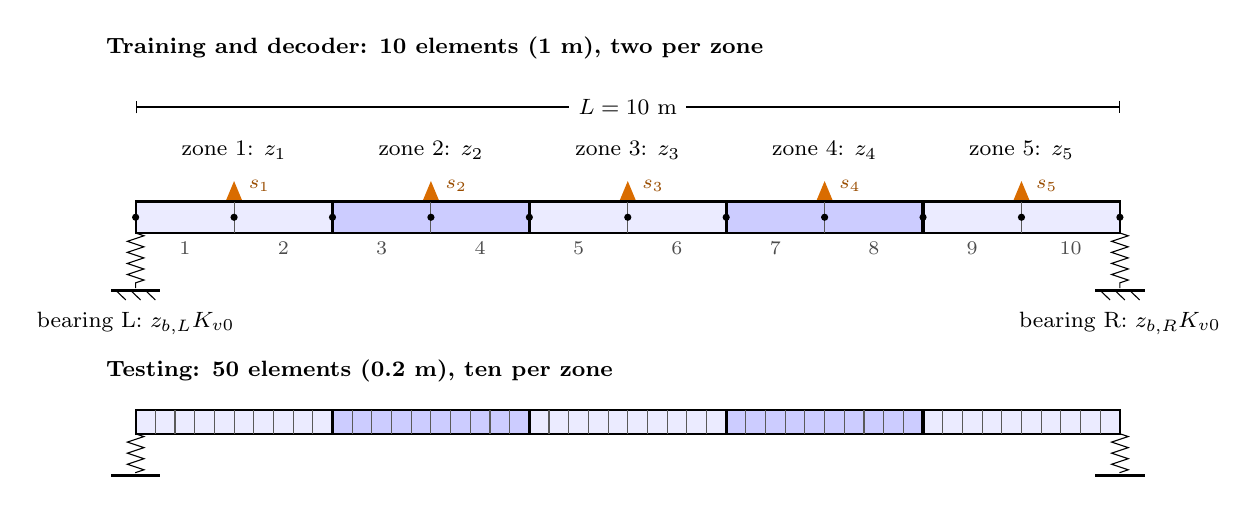
\begin{tikzpicture}[>=Stealth,font=\small,x=1.25cm,y=1cm]
  % ---- model used for training (decoder): 10 elements, 5 zones ----
  \node[anchor=west,font=\footnotesize\bfseries] at (-0.4,2.35) {Training and decoder: 10 elements (1~m), two per zone};
  \foreach \i/\c in {0/blue!8,1/blue!20,2/blue!8,3/blue!20,4/blue!8}{
    \fill[\c] (2*\i,0) rectangle (2*\i+2,0.4);
    \node[font=\footnotesize] at (2*\i+1,1.05) {zone \the\numexpr\i+1\relax: $z_{\the\numexpr\i+1\relax}$};
  }
  \draw[thick] (0,0) rectangle (10,0.4);
  \foreach \x in {1,3,5,7,9} \draw[gray!70!black] (\x,0) -- (\x,0.4);
  \foreach \x in {2,4,6,8} \draw[very thick] (\x,0) -- (\x,0.4);
  \foreach \x in {0,...,10} \fill (\x,0.2) circle (1.3pt);
  \foreach \e in {1,...,10} \node[font=\scriptsize,gray!60!black] at (\e-0.5,-0.2) {\e};
  \foreach \x/\k in {1/1,3/2,5/3,7/4,9/5}{
    \fill[orange!85!black] (\x-0.08,0.42) -- (\x+0.08,0.42) -- (\x,0.66) -- cycle;
    \node[font=\scriptsize,orange!60!black,anchor=west] at (\x+0.05,0.6) {$s_{\k}$};
  }
  \draw[|-|] (0,1.6) -- (10,1.6) node[midway,fill=white,font=\footnotesize] {$L=10$~m};
  \foreach \x/\lab in {0/{L},10/{R}}{
    \draw[decorate,decoration={zigzag,segment length=4,amplitude=3}] (\x,0) -- (\x,-0.7);
    \draw[thick] (\x-0.25,-0.73) -- (\x+0.25,-0.73);
    \foreach \h in {-0.2,-0.05,0.1} \draw (\x+\h,-0.73) -- (\x+\h+0.1,-0.85);
    \node[font=\footnotesize,anchor=north] at (\x,-0.88) {bearing \lab: $z_{b,\lab}K_{v0}$};
  }
  % ---- model used for testing: 50 elements ----
  \node[anchor=west,font=\footnotesize\bfseries] at (-0.4,-1.75) {Testing: 50 elements (0.2~m), ten per zone};
  \fill[blue!8] (0,-2.55) rectangle (2,-2.25); \fill[blue!20] (2,-2.55) rectangle (4,-2.25); \fill[blue!8] (4,-2.55) rectangle (6,-2.25);
  \fill[blue!20] (6,-2.55) rectangle (8,-2.25); \fill[blue!8] (8,-2.55) rectangle (10,-2.25);
  \draw[thick] (0,-2.55) rectangle (10,-2.25);
  \foreach \k in {1,...,49} \draw[gray!70!black] (\k*0.2,-2.55) -- (\k*0.2,-2.25);
  \foreach \x in {2,4,6,8} \draw[very thick] (\x,-2.55) -- (\x,-2.25);
  \foreach \x in {0,10}{
    \draw[decorate,decoration={zigzag,segment length=4,amplitude=3}] (\x,-2.55) -- (\x,-3.05);
    \draw[thick] (\x-0.25,-3.08) -- (\x+0.25,-3.08);
  }
\end{tikzpicture}
\caption{FE model of the revised case study (bridge S10 of Moliner et al., 2017, on elastic bearings). Top: model used for
training and embedded in the decoder, with 10 Euler--Bernoulli elements (numbered; dots mark the nodes), two per damage
zone. Bottom: finer model used to generate the test data, with 50 elements, ten per zone; the damage of a
damaged zone is concentrated in some of its elements (R1.5). The seven latent
variables are the stiffness factors of the five 2~m damage zones ($z_1,\dots,z_5$) and of the two bearings ($z_{b,L}$,
$z_{b,R}$), which scale the vertical springs $K_{v0}$. Five accelerometers ($s_1,\dots,s_5$) are placed at the centres of
the zones.}
\label{fig:bridge}
\end{figure}

\begin{table}[H]
\centering\small
\caption{Nominal values of the revised case study and their origin.}
\label{tab:specs}
\footnotesize
\begin{tabular}{p{3.0cm}p{6.6cm}p{5.0cm}}
\toprule
Item & Value & Origin \\
\midrule
Deck & reinforced concrete slab, span $L=10$~m, width $B=11.6$~m, depth $h=0.77$~m & bridge S10, Moliner et al.\ (2017), Table 2 \\
Elastic modulus & $E=3.4849\times10^{10}$~Pa & Moliner et al.\ (2017), Table 3 \\
Mass & 31\,301~kg/m (including ballast, sleepers and rails) & Moliner et al.\ (2017), Table 2 \\
Bending stiffness & $EI=1.54\times10^{10}$~N\,m$^2$, with $I=Bh^3/12$ & from the values above \\
Bearings & vertical springs, $\kappa=0.05$: $K_{v0}=9.5\times10^{6}$~kN/m each; free end rotations & $\kappa$: Moliner et al.\ (2017); range of
commercial bearings and free rotations: Erduran et al.\ (2022) \\
Discretization & 10 elements (training and decoder); 50 elements (test set B) & this work \\
\bottomrule
\end{tabular}
\end{table}

\begin{action}
New FE model of the bridge on elastic bearings \lines{xx--yy}, with Fig.~\tbd{x} (Fig.~\ref{fig:bridge}) and
Table~\tbd{x} (Table~\ref{tab:specs}).
\end{action}

% -----------------------------------------------------------------------------
\begin{rcomment}{3}
Methodology. Another limitation is the damage parametrization presented as a ``local'' loss of stiffness distributed within an element of a specific length. Considering the type of the bridge, this type of damage parametrization is not realistic, neither for steel bridges nor for RC. This point seems particularly important as the novelty of the proposed
methodology is presented as capturing the interconnectedness of damage scenarios. I recommend, in line with the comment above, including the support conditions in the formulation, which can enable to detect damage observed there.
\end{rcomment}

\begin{response}
We have revised the formulation in two ways.

\textit{Support conditions.} As recommended, the support conditions are now part of the formulation: the elastic bearings
are represented by vertical springs at both ends of the deck, each with its own stiffness reduction factor (R2.2,
Fig.~\ref{fig:bridge}), so that damage at the supports can be identified.

\textit{Damage parametrization.} The damage is no longer the stiffness loss of an individual element, but that of a damage
zone along the deck: the stiffness reduction factor of a zone scales the bending stiffness of all its elements (two in the
model used in training, ten in the testing model), independently of the discretization (Eq.~\eqref{eq:Kz}). This
equivalent stiffness reduction of a region of the deck is the usual representation of damage in vibration-based FE model
updating (Teughels et al., 2002; El-Borgi et al., 2005), and Moliner et al.\ (2017) reduce the elastic modulus of their
slab bridges by 10--20\% to account for cracking. To check this representation when the actual damage is concentrated,
the damage of every damaged zone in test set B is imposed on a group of contiguous elements of a 50-element model, from one
element (0.2~m) to the whole zone (2.0~m), with the same equivalent stiffness of the zone (R1.5, Eq.~\eqref{eq:localized}).
The model used in training cannot represent this localization.

The latent space now contains seven variables, corresponding to the stiffness factors of (i) the five zones along the
bridge deck and (ii) the two bearings (left and right). The new design of experiments (R1.6, Table~\ref{tab:doe}) focuses
on localized damage, i.e., damage at one, two or three of these seven locations, and it also includes healthy structures,
damage at four or five locations, and samples drawn uniformly over the whole parameter space. Every location and every
combination of locations, including combinations of deck and bearing damage, appears the same number of times. The
Gaussian copula captures the dependencies between these variables, e.g., between adjacent zones and between an end zone
and its bearing, which can partly compensate each other.
\tbd{VAE results for the bearings (benchmarks P4, P5 and P9).}
\end{response}

\begin{action}
New parametrization with zone and bearing stiffness factors \lines{xx--yy}; localized damage in the test data
\lines{xx--yy}.
\end{action}

% -----------------------------------------------------------------------------
\begin{rcomment}{4}
Methodology. The numerical case study, 5-elements simply supported beam is too simplistic. I would recommend at least
considering a more realistic case and testing the proposed method on a lab scale beam.
\end{rcomment}

\begin{response}
We agree that the original case study was too simplistic. We have revised it in two ways to bring it closer to a
realistic situation:
\begin{enumerate}[leftmargin=*,label=(\arabic*)]
\item A new FE model of a single-span bridge taken from the literature, discretized into 10 elements and supported on
elastic bearings, represented by vertical springs at both ends (R2.2).
\item The test data are generated with a much finer discretization (50 elements), as a real structure has many more DOFs
than the model embedded in the decoder, and every simulated structure has a perturbed mass (R1.2). The data are thus
generated with models that differ from the one used by the SciML method, as happens when a numerical model is used to
interpret the measurements of a real system.
\end{enumerate}
The validation on a laboratory-scale beam is not included in this revision. We now state it clearly as a limitation of the
present work, and we propose the validation with data from an experimental benchmark as future work.
\end{response}

\begin{action}
New case study \lines{xx--yy}; limitation and future work stated in the conclusions \lines{xx--yy}.
\end{action}

% =============================================================================
\section{Reviewer \#3}
% =============================================================================

\begin{rcomment}{}
In this manuscript, a novel probabilistic machine learning framework is presented for vibration-based damage
identification in civil infrastructure. The SHM approach employs a physics-informed Gaussian copula variational
autoencoder. The effectiveness of the framework is explored in detail and validated under various damage scenarios
using synthetic, noise-contaminated data of a simply supported bridge. The manuscript contains novel theoretical
developments that are worth publishing. Before publication, the following issues have to be addressed.
\end{rcomment}


% -----------------------------------------------------------------------------
\begin{rcomment}{1}
In Bayesian finite element model updating, the discrepancy between the physical structure and the parameterized
mathematical model (i.e., modeling error) dominates over sensor noise. The current validation assumes a perfectly known
baseline mass matrix and attributes all dynamic discrepancies to stiffness reductions (which are updated in the process)
and artificial Gaussian noise. To demonstrate the robustness of the PI-GCVAE, the authors must explore its sensitivity
to modeling errors (e.g., small random perturbations to the mass matrix) and investigate how such unmodeled dynamics
propagate into the posterior uncertainty bounds for the stiffness reduction factors.
\end{rcomment}

\begin{response}
We agree, and we followed the reviewer's suggestion. In the revised study, the baseline mass matrix is no longer
perfectly known. Every measurement, in the training, validation and test sets, comes from an as-built structure whose
mass differs from the nominal mass used by the decoder: the mass of each 1 m segment is multiplied by $1+\mu_s$, with
$\mu_s\sim\mathcal{N}(0,0.05^2)$ (Eq.~\eqref{eq:asbuilt}). In the second test set, the data also include a finer discretization and localized damage (R1.2).
The decoder keeps the nominal mass matrix, and the realizations of these perturbations are never available to the VAE.

\textit{Propagation into the posterior.} These unmodelled effects enter the inference through the likelihood
(Eqs.~\eqref{eq:discrepancy} and~\eqref{eq:nll}). We estimate their effect on the observations by simulation: the mass
perturbations alone change the frequencies with a standard deviation of 0.91--1.08\% and the mode shapes by up to
$3.5\times10^{-3}$ in $1-\mathrm{MAC}$ (Table~\ref{tab:budget}, Fig.~\ref{fig:budget}). Combined with the measurement
noise, the standard deviation of the log-frequency errors increases from 2.5\% to 2.66--2.72\%, and that of the
mode-shape components from 0.027--0.033 to 0.028--0.044. Since these values define the likelihood, the posterior bounds of the stiffness
factors widen consistently with what the decoder cannot represent, instead of attributing the mass deviations to
stiffness changes with false confidence. The calibration check on independent data confirms that the likelihood
describes the actual deviations (Fig.~\ref{fig:calib}). With this setup, the exact posteriors of the benchmark scenarios
have standard deviations of 0.03--0.13 for the deck zones and 0.03--0.05 for the bearings. Two of the test sets of R1.5
examine what happens when the modelling error is larger than assumed (twice the mass deviations) or
systematic (additional mass not included in the model).
\tbd{Posterior bounds and coverage of the VAE with modelling error; comparison with the exact posterior.}
\end{response}
\authornote{The reviewer states that modelling error dominates over sensor noise; with 5\% mass deviations, the
modelling error ($\approx$1\% on the frequencies; 1.2--1.8\% in test set B) is smaller than the identification noise (2.5\%); discuss this together with the larger
modelling errors of R1.5.}

\begin{action}
New subsection on modelling errors and their propagation \lines{xx--yy}; Table~\tbd{x} and Fig.~\tbd{x}.
\end{action}

% -----------------------------------------------------------------------------
\begin{rcomment}{2}
In the ``Sensitivity to $\gamma$ hyperparameter and model selection'' section, the hyperparameter $\gamma$, which
balances the data likelihood and the prior regularization, is calibrated based on the performance of the model on the
test dataset. This approach compromises the independence of the test set and results in overly optimistic performance
estimates. The optimal value of $\gamma$ must be selected using only the validation dataset. The authors need to
correct this methodological flaw and subsequently report the unbiased performance metrics on the completely unseen test
set.
\end{rcomment}

\begin{response}
We agree. In the revised formulation, $\gamma$ is no longer
a tuned hyperparameter. The data terms of the loss are now the negative log-likelihood of the frequency and mode-shape
errors, with the variances calibrated by simulation (R3.1):
\begin{equation}
\mathrm{NLL}(\z;\m)=\tfrac12\,\mathbf{d}^{\top}\bm{\Sigma}_f^{-1}\mathbf{d}
+\sum_{j=1}^{n_m}\frac{1-\mathrm{MAC}_j(\bm{\Phi},\hat{\bm{\Phi}}(\z))}{2\,s_{v,j}^2},\qquad
\mathbf{d}=\log\f-\mathbf{b}-\log\hat{\f}(\z).
\label{eq:nll}
\end{equation}
With a uniform prior on $\mathcal{S}=[0.45,1]^7$, the loss
\begin{equation}
\mathcal{L}(\bm\theta)=\frac1N\sum_{i=1}^N\Big(\mathbb{E}_{q}\big[\mathrm{NLL}(\z;\m_i)\big]
-\gamma^2\,\mathcal{H}\big[q_{\bm\zeta_{\bm\theta}}(\z|\m_i)\big]\Big)
\label{eq:loss}
\end{equation}
is the negative ELBO for $\gamma=1$ (up to a constant), whose minimizer is the Bayesian posterior within the variational
family; values $\gamma\neq1$ would produce tempered posteriors without a probabilistic interpretation. We
therefore fix $\gamma=1$ a priori. The trained model is selected on the validation set: we keep the weights with the
lowest negative ELBO, after a warm-up of 150 epochs in which the weight of the likelihood grows from 0.01 to 1. Every 20
epochs, the validation negative ELBO is estimated with 20 samples per observation and the same random numbers each time.
The learning rate, initially $5\times10^{-4}$, is halved after 200 epochs without an improvement larger than 0.002~nats,
and at $10^{-5}$ the same condition stops the training. 
% [ln z omitted in this revision, kept for later] The marginal family is compared with the same validation negative ELBO (R1.4). 
The test sets take no part in these criteria. The performance metrics on test set B are reported in
Table~\ref{tab:metricsB} (R1.3).

\textit{Role of $\gamma$ and sensitivity analysis.} For $\gamma\neq1$, the minimizer of Eq.~\eqref{eq:loss} is the
variational approximation of the tempered posterior $p_\gamma(\z|\m)\propto\exp\big(-\mathrm{NLL}(\z;\m)/\gamma^2\big)\,
p(\z)$: $\gamma<1$ sharpens the posterior (overconfident intervals) and $\gamma>1$ widens it (conservative intervals).
In the revised formulation, the width of the posterior is therefore set by the statistics of the measurement and
modelling errors in the likelihood (R1.2, R1.3), not by $\gamma$. To show this, and to document how sensitive the
results are to this choice, we add a sensitivity analysis in which the model is retrained with
$\gamma\in\{0.5,0.75,1,1.5,2\}$ ($\gamma^2$ from 0.25 to 4), all other settings unchanged. For each value we report,
on the validation set only, the empirical coverage and the MACE of the credible intervals, the error of the posterior
mean, and the agreement with the exact posteriors computed with the same $\gamma$. We expect the posterior means to be
almost insensitive to $\gamma$ and the coverage to be closest to its nominal value at $\gamma=1$. This analysis
illustrates the effect of $\gamma$ and is not used to select it: $\gamma=1$ is kept for all the reported results.
\tbd{Results of the sensitivity analysis: coverage and MACE vs.\ $\gamma$ (figure), error of the posterior mean.}
\end{response}
\authornote{(i) Sensitivity study not run yet: 4 additional trainings ($\gamma=0.5$, 0.75, 1.5, 2). (ii) The submitted
manuscript reports $\gamma=0.30$ (confirmed with manuscript\_old.tex and the archived run Beta0.3), and its selection
relied on MSE, MAE and coverage values affected by the array-shape error described in R1.3. (iii) Test set B is misspecified (localized damage, R1.5), and $\gamma$ slightly above 1 may calibrate better
there (power/generalized posteriors, e.g., Gr\"unwald and van Ommen, 2017). If we want to discuss this, we need a
validation set generated like test set B, so that the test sets are still not used for any choice. }
% (iv) During
% development we inspected test-set results of several marginal families, and the idea of working in $\ln z$ came from best
% fits to the exact marginals of test set A. The criterion written here is validation-only, but we cannot claim that the
% test sets were seen only once or call the metrics fully unbiased; decide how to state this.
%}

\begin{action}
Section ``Sensitivity to $\gamma$ hyperparameter and model selection'' rewritten \lines{xx--yy}.
\end{action}

% -----------------------------------------------------------------------------
\begin{rcomment}{3}
Within the Bayesian setting, the posterior is heavily dependent on the choice of the prior $p(\z)$. The formulation
assumes a bounded uniform prior $\mathcal{U}[0.5,1.0]$. At the same time, the synthetic training dataset is generated
by uniformly sampling the same space. In actual SHM applications, severe damage is highly improbable; thus, a realistic
prior should strongly penalize large reductions in stiffness. The authors should clarify the distinction between the
generative sampling density used for training (which might be uniform to prevent class imbalance) and the theoretical
Bayesian prior incorporated in the ELBO loss. Can the current framework accommodate an informative, non-uniform prior
while training on uniform data? A brief discussion on this decoupling is necessary.
\end{rcomment}

\begin{response}
We now discuss this point explicitly. Two different distributions play a
role:
\begin{itemize}[leftmargin=*]
\item The \emph{prior} $p(\z)$ is part of the Bayesian model. It enters the loss through the negative ELBO of each
observation,
\begin{equation}
-\mathrm{ELBO}(\m)=\mathbb{E}_q\big[\mathrm{NLL}(\z;\m)\big]+\mathbb{E}_q\big[\log q(\z|\m)\big]
-\mathbb{E}_q\big[\log p(\z)\big],
\label{eq:elbo_prior}
\end{equation}
and through the reference posterior.
\item The \emph{sampling density} of the training data (the DoE) only determines which observations the encoder sees
during training. The loss is an average over observations of Eq.~\eqref{eq:elbo_prior}, and for each observation its
minimizer is the posterior $p(\z|\m)\propto p(\m|\z)\,p(\z)$, independently of how often that observation appears in the
training set. The DoE therefore determines where the amortized encoder is accurate, not which posterior it targets.
\end{itemize}
The revised study makes this decoupling explicit: the prior is uniform on $[0.45,1]^7$, whereas the DoE is a balanced
mixture of healthy and localized damage scenarios (R1.6) that is far from uniform (two thirds of the parameters lie in
$[0.95,1]$). For a uniform prior, the last term of Eq.~\eqref{eq:elbo_prior} is constant, which is why the loss only
contains the likelihood and the entropy. An informative prior, e.g., one that penalizes large stiffness reductions,
only requires adding $-\mathbb{E}_q[\log p(\z)]$ to the loss, estimated with the same samples of $q$, and using the same
prior in the reference posterior. Neither the training data nor the architecture change.
\end{response}
\authornote{optional: demonstrate an informative prior on one benchmark.}

\begin{action}
New paragraph on the prior and the sampling density of the training data \lines{xx--yy}, with
Eq.~\eqref{eq:elbo_prior}.
\end{action}

% -----------------------------------------------------------------------------
\begin{rcomment}{4}
The identification relies on the first 5 modes to estimate damage in a 5-element beam. The accuracy of Bayesian
parameter estimation is fundamentally dictated by the information content of the measured data. While higher modes
offer better spatial resolution for localized damage, they are increasingly contaminated by measurement noise. A brief
sensitivity analysis or discussion of how the number of modes used affects parameter identifiability and the width of
the posterior uncertainty bounds is needed. How does the proposed VAE handle the transition to a severely ill-posed
scenario when fewer modes are available?
\end{rcomment}

\begin{response}
We agree, and we carried out a sensitivity analysis of the measurement setup with the data generator of the revised
study.

\textit{Distinguishability of the modes.} The modes must be distinguishable at the sensors, otherwise they cannot be
paired with those of the model. Over random damage states, the largest MAC between two different modes at the sensors is
0.24 for the six sensors at the zone boundaries of the submitted version and 0.07 for five sensors at the
zone centres, which we adopt.

\textit{Exact posteriors.} For five setups, we computed the exact posteriors of five benchmark scenarios, each setup with
its own calibrated likelihood (Table~\ref{tab:modes}). With fewer modes, the posteriors widen (mean standard deviation
0.046--0.075 with five modes and 0.062--0.088 with three), and the probability assigned to the true damage location
decreases. For the severe damage of zone 1 in P1 ($z_1=0.56$), the posterior probability that zone 1 is damaged ($z_1<0.85$) is 1.00 with five modes,
0.87 with three modes and 0.77 with three modes and three sensors, while that of its mirror zone grows from 0.08 to 0.34 and 0.50. In P9, the mirror
probability is 0.39, 0.26 and 0.49, so it does not vary monotonically in a single noise realization. The transition to ill-posedness therefore appears as wider and skewed marginals and more ambiguity between
symmetric locations. The bearing of P4 remains identified in all setups (standard deviation 0.022--0.052), because the bearings affect every mode.

\textit{Adopted setup.} We adopted five vertical accelerometers at the zone centres and the first five modes (up to
155~Hz for the healthy bridge), in which the modes are well separated at the sensors and the mesh error of the decoder is small
(Table~\ref{tab:mesh}). With this setup, the posteriors keep a substantial uncertainty (standard deviations up to 0.13 for the deck zones), so the
identification is genuinely probabilistic.

\textit{The VAE with less information.} To show how the VAE handles fewer data, we also train it with three modes and,
with five modes, with the frequencies only. 
% Before training, we checked the marginal family against the exact posteriors
% of 131 test scenarios (best fit of each marginal, without the encoder). The mean Wasserstein-1 distance of one Gaussian in
% $\ln z$ to the exact marginals is 0.0013 with five modes, 0.0023 with three modes and 0.0021 with the frequencies only;
% for one Gaussian in $z$, it is 0.0033, 0.0053 and 0.0048.
\tbd{Comparison between the VAE and the exact posteriors with five modes, three modes and frequencies only.}
\end{response}

\begin{table}[H]
\centering\small
\caption{Exact posteriors of benchmarks P1, P3, P4, P6 and P9 for five measurement setups (one noise realization per
setup; calibrated likelihood of each setup): range of the mean posterior standard deviation and of the widest 95\%
credible interval over the benchmarks, and posterior probability that the true damaged parameter and its mirror have
$z<0.85$ (P1: zone 1, true $z_1=0.56$, mirror zone 5; P4: left bearing, true $z_{b,L}=0.55$, mirror right bearing; P9:
zone 2, true $z_2=0.58$, mirror zone 4).}
\label{tab:modes}
\footnotesize\setlength{\tabcolsep}{4pt}
\begin{tabular}{lccccc}
\toprule
 & & Widest 95\% & \multicolumn{3}{c}{Probability of $z<0.85$: true / mirror} \\
\cmidrule(l){4-6}
Setup & Mean std & interval & P1 & P4 & P9 \\
\midrule
7 sensors (with supports), 5 modes & 0.042--0.065 & 0.24--0.37 & 0.999 / 0.235 & 1.000 / 0.006 & 1.000 / 0.215 \\
5 sensors, 5 modes (adopted) & 0.046--0.075 & 0.25--0.49 & 1.000 / 0.081 & 1.000 / 0.053 & 0.999 / 0.394 \\
5 sensors, 4 modes & 0.051--0.066 & 0.24--0.45 & 1.000 / 0.165 & 1.000 / 0.028 & 0.999 / 0.056 \\
5 sensors, 3 modes & 0.062--0.088 & 0.34--0.50 & 0.868 / 0.337 & 1.000 / 0.167 & 0.962 / 0.261 \\
3 sensors, 3 modes & 0.068--0.104 & 0.36--0.52 & 0.767 / 0.501 & 1.000 / 0.112 & 0.830 / 0.490 \\
\bottomrule
\end{tabular}
\end{table}
\authornote{one noise realization per setup; replicas would smooth non-monotone values such as the mirror probability of
P9. The values come from the script identifiability\_setups.py.}

\begin{action}
New paragraph and table on the influence of the number of modes and sensors \lines{xx--yy}.
\end{action}

% -----------------------------------------------------------------------------
\begin{rcomment}{5}
The readability of the manuscript would benefit from a dedicated flowchart illustrating the synthetic dataset
generation process (parameter sampling, forward eigenvalue solution, noise injection), distinguishing clearly between
the offline training phase and the online inference phase.
\end{rcomment}

\begin{response}
We agree, and we added the flowchart of Fig.~\ref{fig:flowchart}. In the offline phase, the design of experiments gives the
damage states of the training, validation and test sets (R1.6). Each damage state is combined with one new as-built
structure, its modal data are computed with the FE model of that set, and measurement noise is added (R1.1, R1.2). The
likelihood is calibrated separately, with simulated as-built structures, and the VAE is trained with the nominal decoder
without ever using the true damage states in the loss. In the online phase, the trained encoder maps the measured modal
data directly to the approximate posterior; neither the decoder nor new simulations are needed.
\end{response}

\begin{figure}[H]
\centering
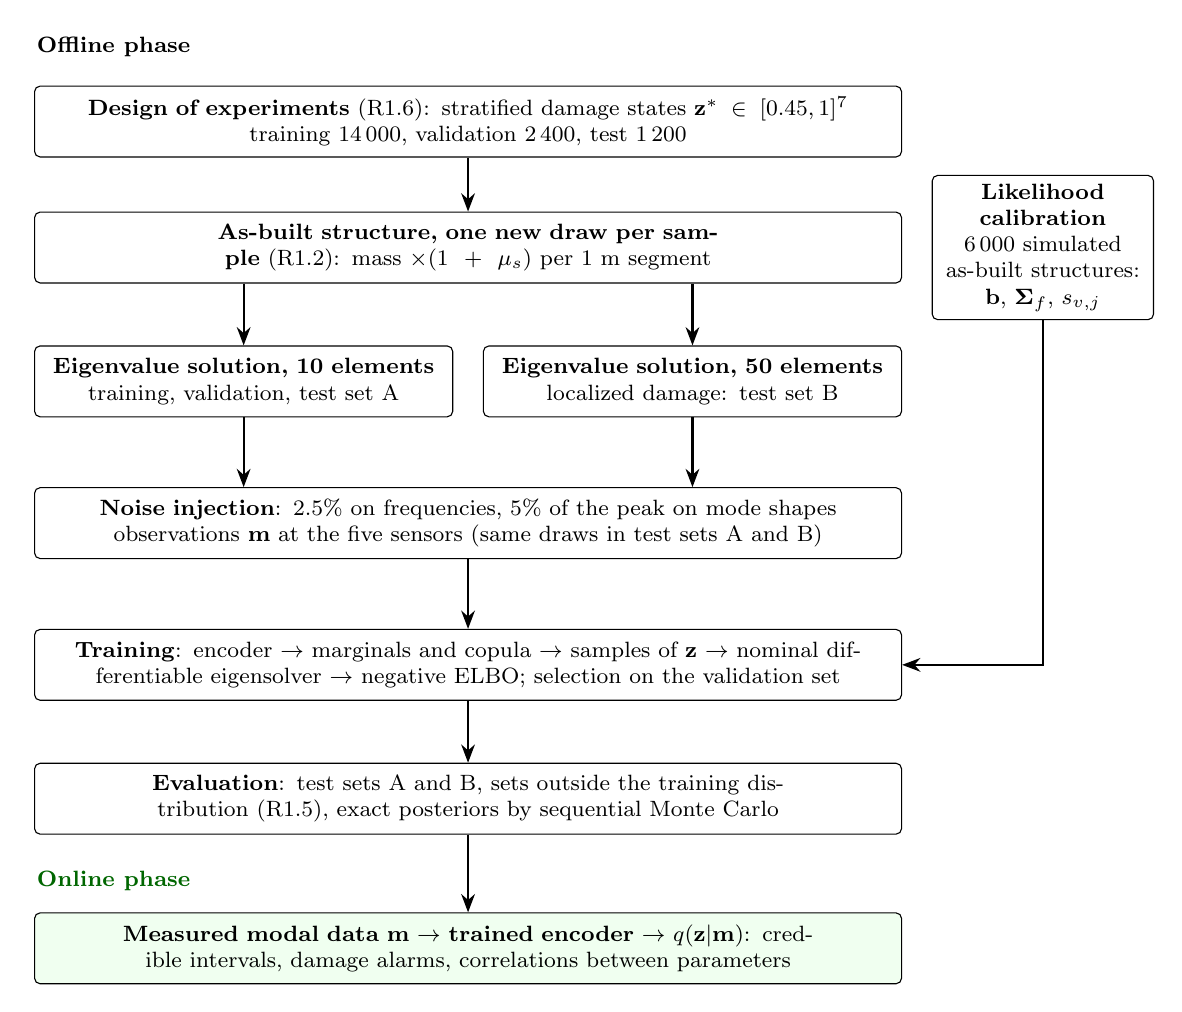
\begin{tikzpicture}[>=Stealth,font=\footnotesize,
  box/.style={draw,rounded corners=2pt,align=center,minimum height=0.9cm,fill=white,inner sep=3pt},
  arr/.style={->,thick}]
  \node[anchor=west,font=\bfseries\footnotesize] at (-5.6,0.95) {Offline phase};
  \node[box,text width=10.8cm] (doe) at (0,0) {\textbf{Design of experiments} (R1.6): stratified damage states $\z^*\in[0.45,1]^7$\\training 14\,000, validation 2\,400, test 1\,200};
  \node[box,text width=10.8cm] (ab) at (0,-1.6) {\textbf{As-built structure, one new draw per sample} (R1.2): mass $\times(1+\mu_s)$ per 1~m segment};
  \node[box,text width=5.1cm] (fe10) at (-2.85,-3.3) {\textbf{Eigenvalue solution, 10 elements}\\training, validation, test set A};
  \node[box,text width=5.1cm] (fe50) at (2.85,-3.3) {\textbf{Eigenvalue solution, 50 elements}\\localized damage: test set B};
  \node[box,text width=10.8cm] (noise) at (0,-5.1) {\textbf{Noise injection}: 2.5\% on frequencies, 5\% of the peak on mode shapes\\observations $\m$ at the five sensors (same draws in test sets A and B)};
  \node[box,text width=10.8cm] (train) at (0,-6.9) {\textbf{Training}: encoder $\to$ marginals and copula $\to$ samples of $\z$ $\to$ nominal differentiable eigensolver $\to$ negative ELBO; selection on the validation set};
  \node[box,text width=10.8cm] (test) at (0,-8.6) {\textbf{Evaluation}: test sets A and B, sets outside the training distribution (R1.5), exact posteriors by sequential Monte Carlo};
  \node[anchor=west,font=\bfseries\footnotesize,green!40!black] at (-5.6,-9.65) {Online phase};
  \node[box,text width=10.8cm,fill=green!6] (on) at (0,-10.5) {\textbf{Measured modal data} $\m$ $\to$ \textbf{trained encoder} $\to$ $q(\z|\m)$: credible intervals, damage alarms, correlations between parameters};
  \node[box,text width=2.6cm] (cal) at (7.3,-1.6) {\textbf{Likelihood calibration}\\6\,000 simulated as-built structures: $\mathbf{b}$, $\bm{\Sigma}_f$, $s_{v,j}$};
  \draw[arr] (doe)--(ab);
  \draw[arr] (fe10 |- ab.south)--(fe10.north);
  \draw[arr] (fe50 |- ab.south)--(fe50.north);
  \draw[arr] (fe10.south)--(fe10 |- noise.north);
  \draw[arr] (fe50.south)--(fe50 |- noise.north);
  \draw[arr] (noise)--(train);
  \draw[arr] (train)--(test);
  \draw[arr] (cal.south) |- (train.east);
  \draw[arr] (test)--(on);
\end{tikzpicture}
\caption{Generation of the synthetic data, offline training and evaluation, and online inference.}
\label{fig:flowchart}
\end{figure}

\begin{action}
New flowchart (Fig.~\tbd{x}, Fig.~\ref{fig:flowchart}) \lines{xx--yy}.
\end{action}

% -----------------------------------------------------------------------------
\begin{rcomment}{6}
Equation 11 ($\mathcal{L}_{\mathrm{freq}}$): The notation $\mathbf{K}_{\mathrm{G}}$ in the decoder function is slightly
confusing since Eq. 5 defines $\hat{\mathbf{K}}_{\mathrm{G}}(\z)$ as the updated stiffness matrix. Please clarify if
$\mathbf{K}_{\mathrm{G}}$ refers to the baseline assembled matrix to avoid confusion with the damaged global matrix.
\end{rcomment}
\pending

% -----------------------------------------------------------------------------
\begin{rcomment}{7}
Sample size in training ($H=1$): In the ``Architecture design and training specifications'' section, it is stated that
a single sample ($H=1$) is drawn during training. While common in VAEs with large batch sizes, please briefly justify why
$H=1$ is sufficient to approximate the expectations in the ELBO loss.
\end{rcomment}

\begin{response}
In the revised implementation, we draw $H=6$ samples of the approximate posterior per observation. With batches of 256
observations, each gradient step uses 1\,536 samples. The Monte Carlo estimate of the loss is unbiased for any $H$, and
$H$ only affects the variance of the gradients. This variance is further reduced because the entropy is computed
exactly, in closed form (Eq.~\eqref{eq:loss}), so that the samples are only used for the expectation of the negative
log-likelihood. The samples are obtained with the closed-form quantile of the truncated normal distribution at the uniform
variables produced by the Gaussian copula. This expression is differentiable with respect to the encoder outputs, and it
replaces the rejection sampling of the submitted version.
% $H$ only affects the variance of the gradients. This variance is further reduced because the entropy is computed
% exactly, in closed form (Eqs.~\eqref{eq:marginal} and~\eqref{eq:loss}), so that the samples are only used for the
% expectation of the negative log-likelihood. The samples are obtained with the closed-form quantile of
% Eq.~\eqref{eq:marginal} at the uniform variables produced by the Gaussian copula. This expression is differentiable with
% respect to the encoder outputs, and it replaces the rejection sampling of the submitted version.
\end{response}
\authornote{optional: a short check of the sensitivity of the results to $H$.}

\begin{action}
Training specifications updated \lines{xx--yy}.
\end{action}

% -----------------------------------------------------------------------------
\begin{rcomment}{8}
Hardware and computational cost: Please report the hardware specifications and the approximate wall-clock time
required for the 11,000 training epochs to provide a practical sense of the computational cost of differentiating the
eigenvalue solver.
\end{rcomment}
\pending
\authornote{report the hardware and wall-clock time of the final training on the GPU server (NVIDIA Quadro GV100 and L40S GPUs; the eigenproblems are solved on the CPU in double precision), measured on an otherwise idle GPU.}

% =============================================================================
\section{References cited in this letter}
% =============================================================================
{\small
\begin{itemize}[leftmargin=*,label={}]
\item El-Borgi, S., Choura, S., Ventura, C., Baccouch, M., Cherif, F. (2005). Modal identification and model updating of a reinforced concrete bridge. Smart Struct.\ Syst.\ 1(1), 83--101.
\item Erduran, E., Nordli, C., Gonen, S. (2022). Effect of elastomeric bearing stiffness on the dynamic response of railway bridges considering vehicle--bridge interaction. Appl.\ Sci.\ 12(23), 11952.
\item Luo, L., Sun, L., Song, M., Liu, J., Li, Y., Xia, Y. (2025). Joint load-parameter-response identification using a physics-encoded neural network. Mech.\ Syst.\ Signal Process.\ 230, 112597.
\item Moliner, E., Mart\'{\i}nez-Rodrigo, M.D., Museros, P. (2017). Dynamic performance of existing double track railway bridges at resonance with the increase of the operational line speed. Eng.\ Struct.\ 132, 98--109.
\item Teughels, A., Maeck, J., De Roeck, G. (2002). Damage assessment by FE model updating using damage functions. Comput.\ Struct.\ 80(25), 1869--1879. \tbd{check the volume and pages}
\item \tbd{Refs.~39 and 41 are those of the manuscript (Fernandez-Navamuel et al., 2025; Fernandez-Navamuel et al., 2026).}
\end{itemize}
}

\end{document}
